\documentclass[12pt]{scrreprt}
\usepackage{graphicx}
\usepackage{geometry}
\geometry{
 a4paper,
 left=20mm,
 right=20mm,
 top=25mm,
 headheight=20mm,
 headsep=0mm,
 bottom=30mm,
}
\usepackage[T1]{fontenc}				% Trennung von Umlauten.
\usepackage[ngerman]{babel}	
\usepackage[utf8]{inputenc}
\usepackage[headsepline]{scrlayer-scrpage}
\ModifyLayer[addvoffset=-10pt]{scrheadings.head.below.line}
\usepackage{blindtext}
\usepackage[font=small,labelformat=empty,justification=centering]{caption}
\setlength{\parindent}{0em}

%Autordaten
\newcommand{\datum}{25.06.2020}
\newcommand{\autorinfo}{\textbf{Wechler, Tim-Jonas} (1137877)}


\ihead{\textbf{WT 1} \datum}
\chead{\autorinfo}
\ohead{\vspace{10pt}
\includegraphics[width=4cm]{logo_simple}}
 
\begin{document}

Bei der letzten Vorlesung vom 25.06.2020 ging es um die thermische aktivierte Vorgänge und das Eisen-Kohlenstoffdiagramm.\medskip

In den thermisch aktivierten Vorgängen gibt es die \textbf{Diffusion}. Unter diesem versteht man ein wandern von Atomen, Molekülen oder Bausteinen über eine Strecke die größer ist als ein Atomdurchmesser.
Diffusion kann auf drei Möglichkeiten statt finden, der Austauschmechnanismus, bei dem die jeweilige Elemente ihre Plätze mit benachbarten austauschen.
Eine andere Möglichkeit der Diffusion ist eine Leerstelle zu besetzen. Die letzte Möglichkeit der Diffusion ist der Zwischengittermechanismus, hierbei finden Bewebungen zwischen den der Gitterstruktur statt.\smallskip

Die Diffusion unterscheidet sich in drei Arten, die oberflächen Diffusion, die korngrenzen Diffusion und die Gitter-Diffusion. Mit einer fallenden Temperatur sinkt die mögliche zurücklegende Strecke. Bei der Oberflächen-Diffusion wandern die Atome, Moleküle oder Bausteine am weitesten, da sie zu einer Seite theoretische eine unendliche Leerstelle haben.
Die nächste Art mit einer mittleren Entfernung ist die Diffusion entlang der Korngrenzen. Die Diffusion mit der geringsten Entferung ist die Gitter-Diffusion.\medskip

Zu den thermisch aktivierten Vorgängen wurde uns auch noch die \textbf{Kristallerholung} und die \textbf{Rekristallisation} näher gebracht. 
Im Bezug zur Kristallerholung haben wir erfahren das es sich hier bei um ein ausheilen von Gitterbaufehler handelt.
Bei diesem vorgang wird die Gitterspannungen verringert, die Härte und Zugfestigkeit des Werkstoffs bleibt bestehen. \\
In dem Prozess der Rekristallisation tritt eine Reduzierung der Versetzungsdichte auf was zur Folge hat das die mechanische Eigenschaften sich durch Neubildung und Wachstum versetzungsarmer Kirstalle reduzieren. Der Wachstum läuft ähnlich wie bei den Kristallisatio ab.
Unter Kornwachstum versteht man ein Grenzbewegung die keine Keimbildung voraussetzt. Die Korngrenzen wandern immer von einer niedirgerne Versetzungsdichte zu einer höheren.\bigskip

Als nächstes haben wir über das \textbf{Eisen-Kohlenstoff-Diagramm} gesprochen. Hier wird zwischen drei Werkstoffgruppen unterschieden, Reineisen, Stahl und Gusseisen. 
Reineisen hat keine Kohlenstoffanteil von \(c \leq 0,008\% \;C\). Reineisen ist sehr weich und wird nich als Konstruktionswerkstoff verwendet. Dafür besitzt Reineisen eine hohe magnetischen Permeabilität und ist dadurch gut geeigenet beim Einatz in der Elektrotechnik.
Stahl hat einen Kohlenstoffanteil von \(c \leq 2\%C\) und Gusseisen hat eine Kohlenstoffanteil von \(c = 2 - 4\%C\). Es gibt noch weitere Legierungen die einen Anteil \(\geq 4\%C\) besitzen aber die haben eine keine technische Verwendung.
Typischerweise wird das Eisen-Kohlenstoff-Diagramm bis zu einem Anteil von \(Fe_3C c=6,67\%C\) dargestellt (siehe nächste Seite).\smallskip

Da uns das Eisen-Kohlenstoff-Diagramm in der Vorlesung Fertigungsverfahren schon gezeigt wurde war es nicht direkt etwas neues für mich, dennoch waren die Besonderheiten wie der Bereich um ABHJN und GOPS sehr interessant und durch das vorwissen aus der vergangen Vorlesungsstunden habe ich dieses wesentlich besser verstanden zu lesen. 
In Hinblick auf die Erwähnung von Reineisen, Stahl und Gusseisen ergaben auch die Unterteilungen und Abgrenzung bei OEC einen Sinn und man kann es zuordnen. 
Da hes hier schwer ist auf die Besonderheiten der einzelnen Teilbereichen einzugehen verweise ich auf das Vorlesungs-Skript von Dr.\,E.Geberth, hier findet man eine gute detailierte Auflistung der einzelnen Teilbereiche.\bigskip

Allgemein zusammenfassend habe ich wieder sehr viel neues gelernt, besonders die Diffusion und die Details zum Eisen-Kohlenstoff-Diagramm fande ich sehr aufschlussreich und informativ.








\newpage

\begin{figure}[h]
	% \textwidth bezieht sich nun auf die Minipage
	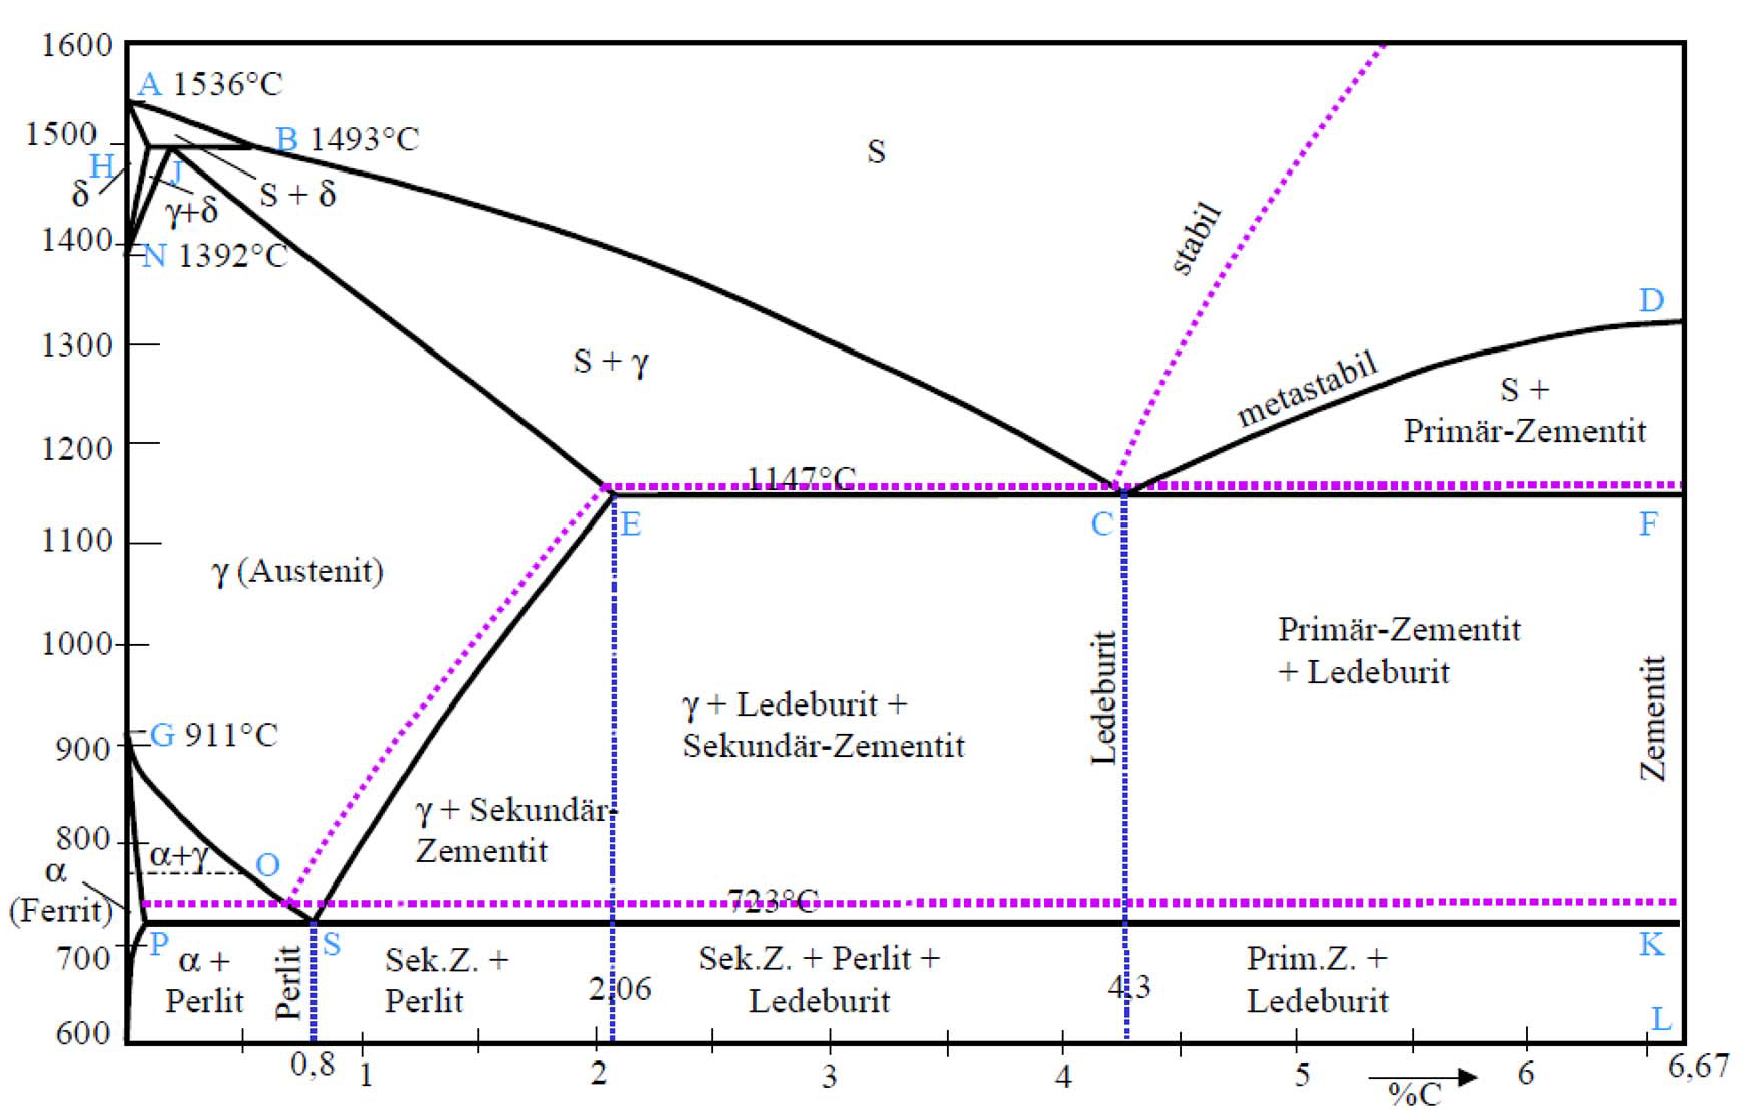
\includegraphics[width=\textwidth]{fec-diagramm.png}
	\caption{Eisen-Kohlenstoff-Diagramm\\(Quelle: Vorlesungsfolien WT1 Dr.\,E.Geberth)}
% \caption{noch eine Caption}
\end{figure}

\end{document}

